\section{Preliminaries} \label{sec:Preliminaries}

\subsection{The \oeis document format}\label{sec:doc-form}

The \emph{internal format} \cite{oeis-help} is line-based in the sense that
each line starts with a marker that represents the kind of content found 
in that line. We briefly introduce the relevant kinds below but refer to 
\cite{oeis-help} for details.

\begin{wrapfigure}{r}{9.5cm}
\vspace{-1.0cm}
\begin{center}
\begin{tabular}{|lll|}
\hline
\req{\textit{Ident.}} & \bbc & $\mathtt{\%I \;} \mathit{ID}\; \opt{M_n} \; \opt{N_n} $ \\
$\mathit{ID}$ & \bbc & Identification number in \cite{oeis} \\
$M_n$ & \bbc & Identification number in \cite{encyc-is} \\
$N_n$ & \bbc & Identification number in \cite{handbook-is} \\
\req{\textit{Values}} & \bbc & $\mathtt{\%S \; } \mathit{ID}\; \mathrm{nr}^\rep \; \opt{\mathtt{\%T \; 
ID}\; \mathrm{nr}^\rep \; \opt{\mathtt{\%U \; } \mathit{ID}\; \mathrm{nr}^\rep}} $ \\

\req{\textit{Name}} & \bbc & $\mathtt{\%N \; } \mathit{ID} \; \mathrm{text}$ \\
\textit{References} & \bbc & $\mathtt{\%D \; } \mathit{ID} \; \mathrm{text}$  \\
\textit{Formula} & \bbc & $\mathtt{\%F \; } \mathit{ID} \; \mathrm{formula}$  \\
\req{\textit{Author}} & \bbc & $\mathtt{\%A \; } \mathit{ID} \; \mathrm{text}$  \\
\textit{Examples} & \bbc & $\mathtt{\%E \; } \mathit{ID} \; \mathrm{text}$ \\
\hline

\end{tabular}
\caption{Grammar of \oeis Internal Format}\label{fig:int-form}
\end{center}
\end{wrapfigure}

\begin{compactenum}
 \item The \emph{identification} line gives the unique ID of the sequence declared in that document. 
 \item The \emph{start values} lines give the beginning of the sequence. It is used for searching as 
well as lexicographic ordering of the sequences.
 \item The \emph{name} line gives the name, a brief description or the definition of the sequence.
 \item The \emph{references} lines contain references to papers which in turn refer to or are concerned with the 
 sequence described in the current document.
 \item The \emph{formula} lines give formulas that define or hold for the sequence described in the current document. 
 The formulas are in plain text ASCII syntax that is similar to {\LaTeX} math markup and can contain text as 
 part of the formula or as comments. Among others, here we find the representing functions and the generating
 functions (starting with \texttt{G.f.}) of the sequence in hand.
 \item The \emph{author} line gives the document author typically containing the name and e-mail address.
 \item The \emph{examples} lines give examples and additional information about the initial terms of the sequences
\end{compactenum}

The actual document-level syntax of the internal format is presented below in Figure \ref{fig:int-form} where
we use \req{$\circ$} for required lines, $\opt{\circ}$ for optional parts, $\circ^\rep$ for repetitions and $\circ_1 
\alt \circ_2$ for alternatives. Moreover we use \textit{italic} for grammar productions, \texttt{typewriter font} for 
fixed syntax and normal font for informal descriptions.

[Fibonacci numbers]\label{ex:internal}
  The article for Fibonacci numbers \cite{oeis-fib} was one of the first entries in the
  \oeis and is one of the most comprehensive.  We will use it as a running example
  throughout the report, although we will heavily trim the document for simplicity by
  presenting here only a few sanitized lines. Listing
  \ref{lst:internal} shows the document with identification, values, name and reference
  lines, followed by three formula lines and the author line.

\begin{lstlisting}[caption=A000045,label=lst:internal,basicstyle=\scriptsize\sf]
%I A000045 M0692 N0256
%S A000045 0,1,1,2,3,5,8,13,21,34,55,89,144,233,377,610,987
%N A000045 Fibonacci numbers: F(n) = F(n-1) + F(n-2) with F(0) = 0 and F(1) = 1.
%D A000045 V. E. Hoggatt, Jr., Fibonacci and Lucas Numbers. Houghton, Boston, MA, 1969.
%F A000045 F(n) = ((1+sqrt(5))^n-(1-sqrt(5))^n)/(2^n*sqrt(5))
%F A000045 G.f.: Sum_{n>=0} x^n * Product_{k=1..n} (k + x)/(1 + k*x). - _Paul D. Hanna_, Oct 26 2013
%F A000045 This is a divisibility sequence; that is, if n divides m, then a(n) divides a(m)
%A A000045 _N. J. A. Sloane_, Apr 30 1991
\end{lstlisting}



\subsection{\omdmmt}

The \mmt language \cite{Rabe:MMTLanguageSystem09} is designed to be applicable to a large collection of declarative
formal base languages and all  \mmt notions are fully abstract in the choice of the base language. For clarification,
 typical base languages are logics, type theories, or programming languages. In \mmt, mathematical knowledge is
 defined in terms of four important
units: documents, modules, symbols and objects. The biggest unit of mathematical knowledge, the document, is
represented in  \mmt as a theory graph.
\textbf{Theory Graph} is one of the central notions of  \mmt which contains \emph{theories} or modules and
\emph{views} (morphisms between theories). To understand this better we will define some additional notions. \\
\textbf{Theories} are defined by a set of typed \textbf{symbols} (the signature) and a set of \textbf{axioms}
describing the properties of the symbols. \\
\textbf{Symbols} are either constant declarations (declaring constants, type axioms, lemmas, definitions) or a
structure declaration (which declares an import from another theory). In the latter case, all the symbols from the
imported theory become available. In the theory graph this is represented by an arrow from the imported theory to the importing one.
A \textbf{signature morphism} $\sigma$ from a source theory \emph{S} to a target theory \emph{T} translates or
interprets the symbols of \emph{S} in \emph{T}. \\
If we have entailment relations for the formulas of S and T, a signature morphism that translates all theorems of
\emph{S} to theorems of \emph{T} is called a \textbf{view}. So, in  \mmt a \textbf{view} from \emph{S} to \emph{T} is
 a list of assignments $c \mapsto \omega$ where $c$ is an \emph{S}-constant (axiom) and $\omega$ is a \emph{T}-term
 (proof). This list of assignments induces a homomorphic translation of S-terms to T-terms by replacing every $c$
 with the corresponding $\omega$.   \\
The object level provides the structure of the symbols inside a theory; objects are terms
produced by a grammar in which the basic units are constants, variables, applications and bindings. 

Let us consider the theories (Fig. \ref{img:graph}) of \textbf{group, monoid} and \textbf{unital set} of a monoid and
 one view \textbf{m} which shows that the unital set of a monoid is a group.

\begin{figure}[h!] 
\centerline{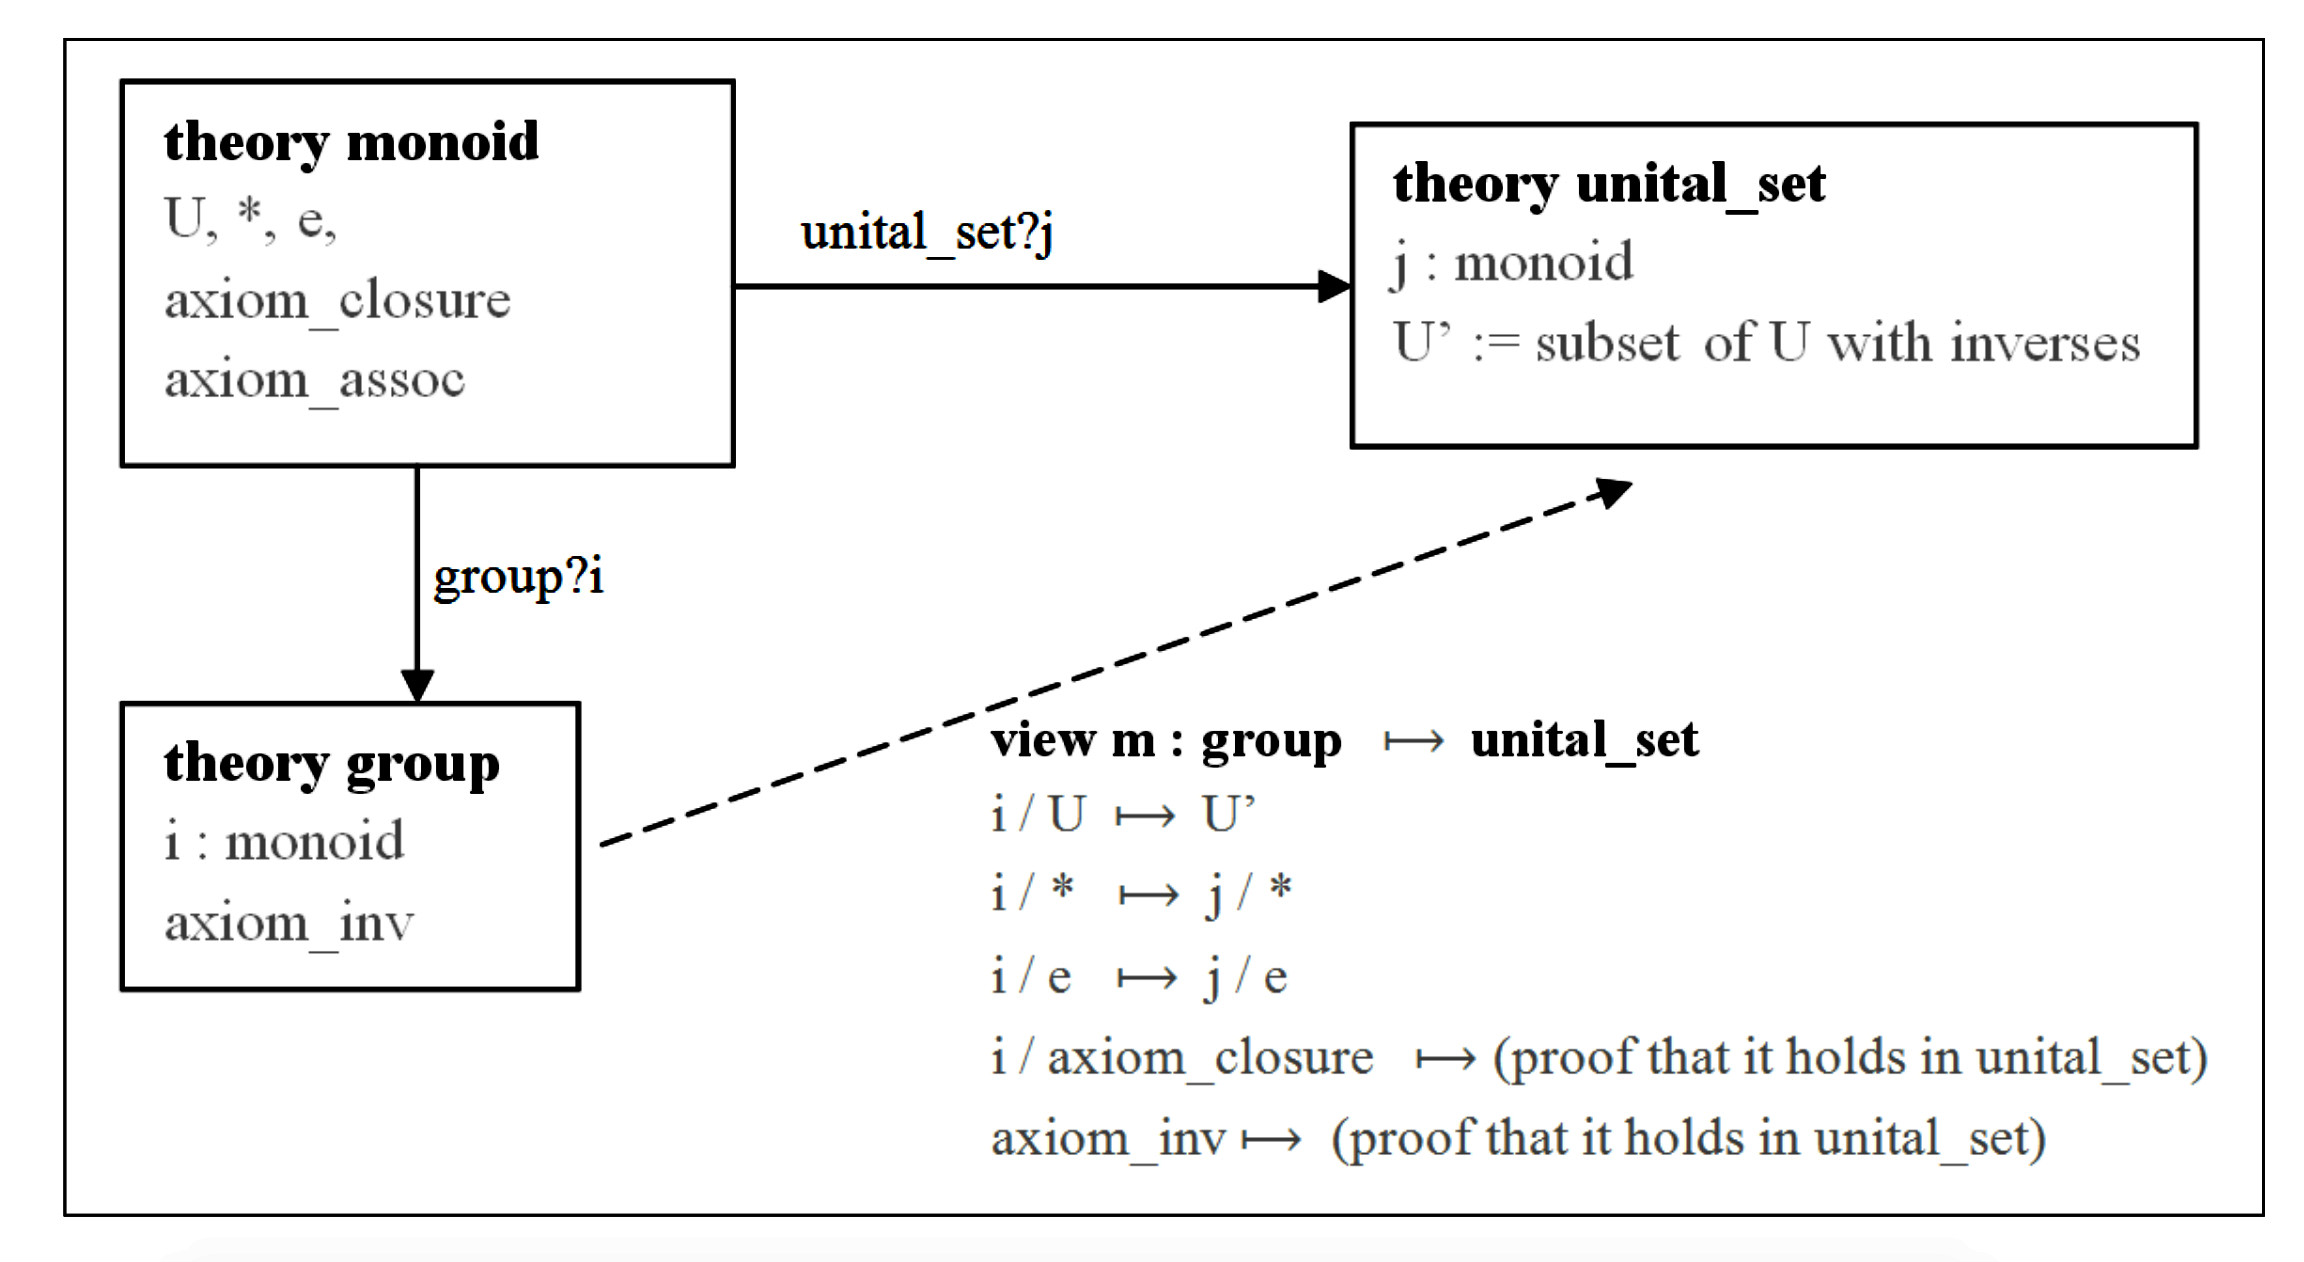
\includegraphics[scale=0.15]{theories1}}
\caption{An Example Theory Graph Comprising Three Theories \label{img:graph}}
\end{figure}

The imports (\textbf{unital\_set?j} and \textbf{group?i}) are marked by solid arrows. Each import carries all the
symbols from the source theory to the destination. In theory \textbf{monoid} the declared constants are
\textbf{U}-underlying set, $*$-monoid operation, \textbf{e}-unity element and \textbf{axiom\_closure, axiom\_assoc}.

Theory \textbf{group} imports from monoid via the structure \textbf{i} and formulates the axiom of invertibility.
Theory \textbf{unital\_set} imports from monoid via \textbf{j} and declares \textbf{U'}-the set of invertible
elements in \textbf{U}.
The view \textbf{m} is mapping all the symbols and proving the axioms still hold with the new mapping in
\textbf{unital\_set}.

\omdoc \cite{Kohlhase:OMDoc1.2} is a content markup format and data model for mathematical documents. It models
mathematical content using three levels.
\begin{compactdesc}
\item[Object Level:] uses {\openmath} and {\mathml} as established standards for
  the markup of \emph{formulae}.
\item[Statement Level:] supplies original markup for explicitly representing the
  various kinds of mathematical statements including \emph{symbol declarations} and \emph{definitions} (which
  introduce
a new symbol names), \emph{assertions} (which can represent theorems, lemmas or corollaries), and \emph{examples}.
\item[Theory Level:] offers original markup that allows for clustering sets
  of statements into \emph{theories} as well as specifying relations between them
  (inclusions, morphisms).
\end{compactdesc}
% \textbf{\omdoc} concentrates on the structural relations between these mathematical
% concepts. It deliberately avoids fixing language primitives for them and abstracts from
% specific mathematical foundations. This is a crucial design choice that makes {\omdoc} a
% universal representation format while remaining manageably simple.

The \mmt \cite{RabKoh:WSMSML13} language can be seen as a restricted version of \omdoc but
with a fully specified semantics. Additionally, for \mmt there is an \mmt system
\cite{Rabe:MAGMS13} which is a Scala-based \cite{scala:webpage} open source implementation
of the {\mmt} language. The key features of the \mmt system for this report are that it
provides an infrastructure for writing importers from any compatible format into \mmt as
well as exporters from \mmt, most notably into (\mathml-enriched) \html for both local and
web-based presentation.

For the sake of simplicity, we often do not differentiate between \mmt and \omdoc
languages in the following and refer to \cite{Kohlhase:OMDoc1.2} and, respectively,
\cite{RabKoh:WSMSML13} for details on each language. Throughout this report we will use
\omdmmt to refer to both \omdoc and \mmt.

\subsection{Theory of Generating Functions}
Generating functions are used to represent sequences efficiently by coding the terms of a sequence
as coefficients of powers of a variable $x$ in a formal power series.
Unlike an ordinary series, this formal series is allowed to diverge, meaning that the generating function is not
always a true function and the "variable" is actually an indeterminate.

Generating functions are used for solving combinatorial problems, recurrences and most importantly in our context,
analyzing various properties of sequences. There are different types of generating functions, including
\textbf{ordinary generating functions, exponential generating functions, Lambert series, Bell series}, and
\textbf{Dirichlet series}.

The \textbf{ordinary generating function} (or just \textbf{generating function}) of a sequence \\ $a_0, a_1, a_2
\ldots, a_{n-1}, a_n, \ldots$ is the infinite series:
\begin{equation}
GF(x) = a_0 + a_1x + a_2x^2 + \ldots + a_{n-1}x^{n-1} + a_nx^n + \ldots = \sum_{i=0}^{\infty} a_ix^i
\end{equation}

For example, the sequence $(1,1,1,1,1, \ldots)$ can be represented as:
\begin{equation}
1 + x + x^2 + \ldots = \frac{1}{1-x}
\end{equation}
We know that the equation above only holds for $|x|<1$ but we ignore the issues of convergence, as already mentioned.
 Thus, the ordinary generating function of this sequence can be written as $\frac{1}{1-x}$.

Due to this representation, generating functions have some interesting properties which we are going to discuss
shortly. Below are some properties of the ordinary generating functions.

Let $f(x) = \sum_{i=0}^{\infty} a_ix^i$, $g(x) = \sum_{i=0}^{\infty} b_ix^i$, $c \in \mathbb{R}$ and $k \in
\mathbb{Z}$, then
\begin{align}
f(x) + g(x) &= \sum_{i=0}^{\infty} (a_i + b_i) x^i \label{eq:add} \\
cf(x) &= \sum_{i=0}^{\infty} ca_ix^i \label{eq:scale} \\
x^kf(x) &= \sum_{i=0}^{\infty} a_ix^{i+k} \label{eq:shift} \\
\frac{d}{dx}f(x) &= \sum_{i=0}^{\infty} (i+1)a_{i+1}x^i \label{eq:diff} \\
\int f(x) dx &= \sum_{i=0}^{\infty} \frac{1}{i+1}a_ix^{i+1} \label{eq:int}
\end{align}
Equation \ref{eq:add} can be interpreted as adding two generating functions is the same as adding the sequences they
represent term by term. From equation \ref{eq:scale}, multiplying a generating function by some constant is the same
as multiplying each term of the sequence by that same constant. From equation \ref{eq:shift}, multiplying the
sequence by $x^k$ is the same as shifting the sequence to the left ($k<0$) or right ($k>0$). If shifted to the right,
 the new terms added in the beginning are $0$s. From equation \ref{eq:diff}, taking the derivative of a generating
 function is the same as multiplying each term by its index and shifting the sequence to the left by one. From
 equation \ref{eq:int}, taking the integral is the same as dividing each term by its index and shifting the sequence
 to the right by one.


%%% Local Variables:
%%% mode: latex
%%% TeX-master: "../report"
%%% End:
